\documentclass{beamer}
\usepackage{listings}
\usepackage{hyperref}
\hypersetup{ 
	colorlinks=true, %
	linkcolor=blue
}

\setbeamertemplate{blocks}[rounded][shadow=true]

\usetheme{progressbar}
\progressbaroptions{titlepage=normal, frametitle=normal}

\title{git flow - Progmatic SCM for Developers}
\institute{Elektrobit Wireless(2011), Company Confidental}
\author{Lifu Zhang}
\date{}
\logo{
\includegraphics[width=1cm]{../progressbar/linuxfb-logo.png}}

\begin{document}
\setbeamertemplate{background}{
\includegraphics[height=\paperheight]{../progressbar/slide.png}}
%\setbeamertemplate{background}{
\includegraphics[height=\paperheight]{../slide.png}}

\lstset{% general command to set parameter(s)
basicstyle=\scriptsize,
% print whole listing small
keywordstyle=\color{black}\bfseries\underbar,
% underlined bold black keywords
identifierstyle=,
% nothing happens
stringstyle=\color{purple}\ttfamily,
% typewriter type for strings
showstringspaces=false}
% no special string spaces

\maketitle

\section{Outline}
\begin{frame}
  \frametitle{Outline}
  \tableofcontents
\end{frame}

%=====================================================================
\section{Ideal Git Branching}
\begin{frame}
	\frametitle{Develop with develop branch}	
	\begin{columns}[c]
	\column{1.5in}
	\begin{itemize}
		\item master - software releases, only stable code permitted
		\item develop - every commits, encourge more commits
		\item Take advantage of frequent commits, while we still could find stable code
	\end{itemize}
	\column{1.5in}
		\framebox{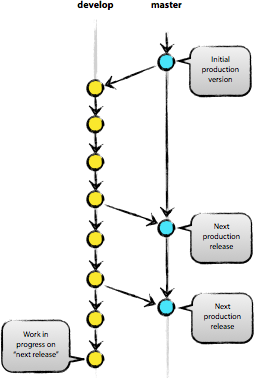
\includegraphics[width=1.5in]{dual-branch}}
	\end{columns}
\end{frame}
%-------
\begin{frame}
	\frametitle{Add feature by feature branch}	
	\begin{columns}[c]
	\column{1.5in}
	\begin{itemize}
		\item Decenteralize the works
		\item Feature could be merge back into develop
		\item A feature could be add in next release
	\end{itemize}
	\column{1.5in}
		\framebox{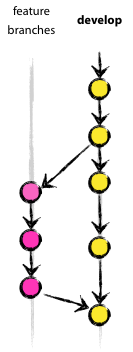
\includegraphics[height=2.5in]{feature-branch}}
	\end{columns}
\end{frame}
%-------
\begin{frame}
	\frametitle{Develop with develop branch}	
	\begin{columns}[c]
	\column{1.5in}
	\begin{itemize}
		\item Bugs occurs everytime
		\item A hotfix should be applied to both develop \& master
		\item A hotfix could be a minor release after merge
	\end{itemize}
	\column{1.5in}
		\framebox{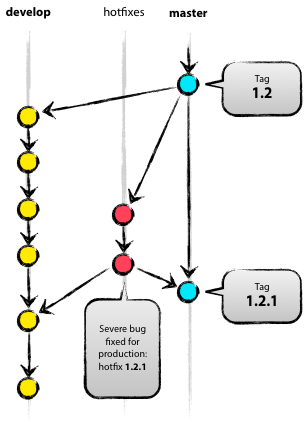
\includegraphics[width=1.5in]{hotfix-branches}}
	\end{columns}
\end{frame}
%-------
\begin{frame}
	\frametitle{Overview of ideal branching}
	\rotatebox{90}{\resizebox{!}{4in}{%
		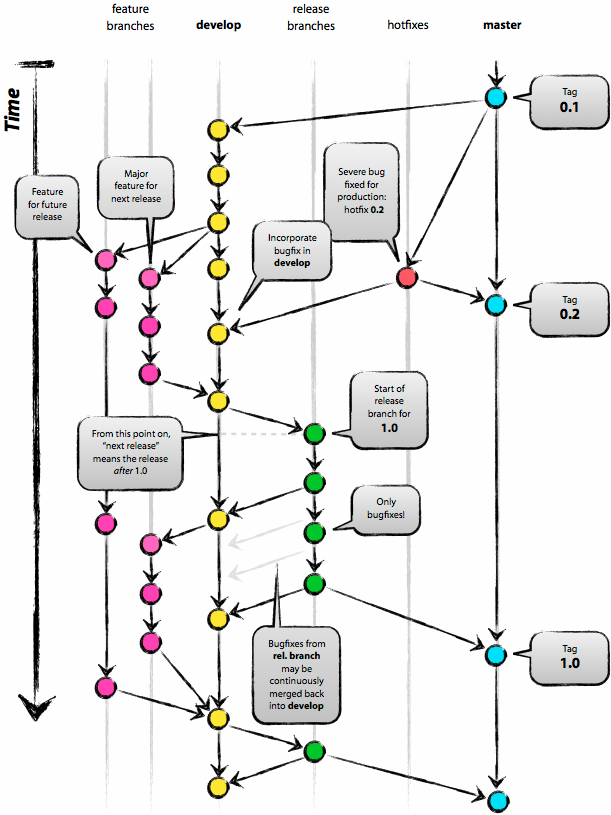
\includegraphics{ideal-git-flow} 
	}}
\end{frame}

%=====================================================================
\section{Git Flow Brief}
\begin{frame}
	\frametitle{gitflow brief}
	Git flow is a module of git, this tool could help us manage code as ''A successful Git branching model'' it only have 4 commands:
	\begin{itemize}
		\item git flow init
		\item git flow feature
		\item git flow release
		\item git flow hotfix
	\end{itemize}
\end{frame}
%-------
\begin{frame}
	\begin{itemize}
		\frametitle{Install gitflow}
		\item Get Git Flow Code from: https://github.com/nvie/gitflow \\
			if you failed at 'git submodule update' run command in your gitflow source directory: \\
			\$sed -i -e ''s:/git:\/\//http:\/\//'' `grep 'git://' -lr .`
		\item \$sudo make [INSTALL\_PRFIX=xxx] install
	\end{itemize}
\end{frame}


%=====================================================================
\section{Using Git Flow}
\subsection{create new feature branches}
\begin{frame}
	\frametitle{Create New Feature}
	\begin{itemize}
		\item git flow feature start xxx
		\item A lots of commits \ldots
		\item git flow feature finish xxx
		\item (if you forget your feature name, you can run \$git flow feature to see it)
	\end{itemize}
	After a feature finish, it will be merged into 'develop'
\end{frame}
%-------
\subsection{relase a new version}
\begin{frame}
	\frametitle{Start a Release}
	\begin{itemize}
		\item git flow release start x.x.x
		\item A lots of comits \ldots
		\item git flow release finish x.x.x
	\end{itemize}
	After rel finish, changes will be merged both into master and develop, and a tag will be created, so the master won't be ahead of develop
\end{frame}
%-------
\subsection{fix bug in released version}
\begin{frame}
	\frametitle{Fix a Bug}
	Bugs occurs every time, after release, we could use git flow hotfix to start a bug fix procedure. \\
	hotfix will be merged to master and develop, and a tag will be generated.

\end{frame}
%-------

%=====================================================================
\section{Reference}
\begin{frame}
	\begin{itemize}
		\item \href{http://jeffkreeftmeijer.com/2010/why-arent-you-using-git-flow/}{Jeff Kreeftmeijer. Why aren't You Using git-flow?}
		\item \href{https://github.com/nvie/gitflow}{Git flow official(host by github)}
	\end{itemize}
\end{frame}

\end{document}

% vim:set fenc=utf8:
% vim:set ft=tex:


